%%%%%%%%%%%%%%%%%%%%%%%%%%%%%%%%%%%%%%%%%
% fphw Assignment
% LaTeX Template
% Version 1.0 (27/04/2019)
%
% This template originates from:
% https://www.LaTeXTemplates.com
%
% Authors:
% Class by Felipe Portales-Oliva (f.portales.oliva@gmail.com) with template 
% content and modifications by Vel (vel@LaTeXTemplates.com)
%
% Template (this file) License:
% CC BY-NC-SA 3.0 (http://creativecommons.org/licenses/by-nc-sa/3.0/)
%
%%%%%%%%%%%%%%%%%%%%%%%%%%%%%%%%%%%%%%%%%

%----------------------------------------------------------------------------------------
%	PACKAGES AND OTHER DOCUMENT CONFIGURATIONS
%----------------------------------------------------------------------------------------

\documentclass[
	12pt, % Default font size, values between 10pt-12pt are allowed
	%letterpaper, % Uncomment for US letter paper size
	%spanish, % Uncomment for Spanish
]{fphw}

% Template-specific packages
\usepackage[utf8]{inputenc} % Required for inputting international characters
\usepackage[T1]{fontenc} % Output font encoding for international characters
\usepackage{mathpazo} % Use the Palatino font

\usepackage{graphicx} % Required for including images

\usepackage{booktabs} % Required for better horizontal rules in tables

\usepackage{listings} % Required for insertion of code

\usepackage{enumerate} % To modify the enumerate environment

%----------------------------------------------------------------------------------------
%	ASSIGNMENT INFORMATION
%----------------------------------------------------------------------------------------

\title{Taller de de modularización con virtualización e Introducción a Docker y a AWS} % Assignment title

\author{Michael Jefferson Ballesteros Coca} % Student name

\date{September 22, 2020} % Due date

\institute{Escuela Colombiana de Ingeniería Julio Garavito \\ Decanatura Ingeniería de Sistemas} % Institute or school name

\class{Arquitecturas Empresariales} % Course or class name

\professor{Luis Daniel Benavides Navarro} % Professor or teacher in charge of the assignment

%----------------------------------------------------------------------------------------

\begin{document}

\maketitle % Output the assignment title, created automatically using the information in the custom commands above

%----------------------------------------------------------------------------------------
%	ASSIGNMENT CONTENT
%----------------------------------------------------------------------------------------


\subsection * {Program Requirements}

\begin {enumerate} [(a \normalfont)]% Sub-questions styled as italic letters
\item The MongoDB service is an instance of MongoDB running in a docker container on an EC2 virtual machine.
\item LogService is a REST service that receives a string, stores it in the database and responds in a JSON object with the last 10 strings stored in the database and the date they were stored.
\item The APP-LB-RoundRobin web application is composed of a web client and at least one REST service. The web client has a field and a button and every time the user sends a message, it is sent to the REST service and updates the screen with the information that it returns in JSON format. The REST service receives the chain and implements a Round Robin load balancing algorithm, delegating message processing and response return to each of the three instances of the LogService service.
\end {enumerate}
% ------------------------------------------------

\subsection * {General}

\subsection * {EC2}

Amazon Elastic Compute Cloud (Amazon EC2) is a web service that provides secure, resizable compute capacity in the cloud. It is designed to make web-scale cloud computing easier for developers. Amazon EC2’s simple web service interface allows you to obtain and configure capacity with minimal friction. It provides you with complete control of your computing resources and lets you run on Amazon’s proven computing environment. Instances:
\begin {itemize}
\item General-Purpose
\item Compute Optimized
\item Memory Optimized
\item Accelerated Computing
\item Storage Optimized
\end {itemize}


% ------------------------------------------------

\subsection * {Docker}


Developing apps today requires so much more than writing code. Multiple languages, frameworks, architectures, and discontinuous interfaces between tools for each lifecycle stage creates enormous complexity. Docker simplifies and accelerates your workflow, while giving developers the freedom to innovate with their choice of tools, application stacks, and deployment environments for each project.


% ------------------------------------------------- ---------------------------------------
\subsection * {Implementation}

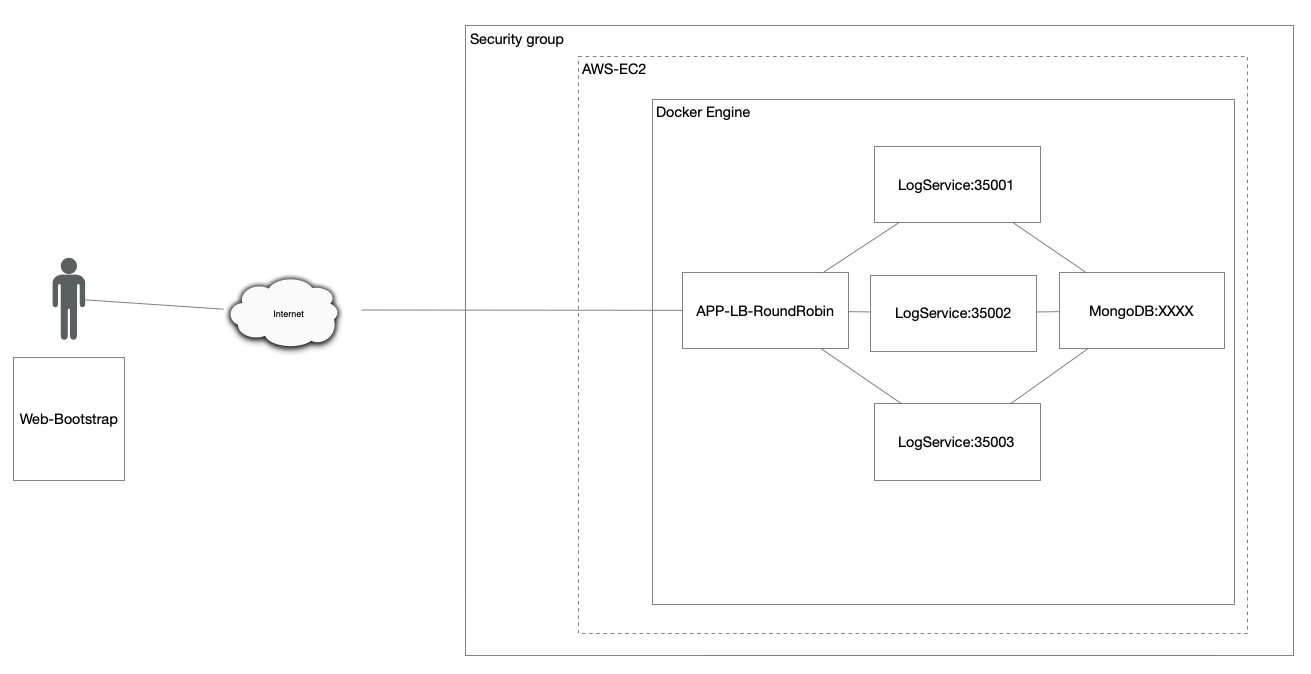
\includegraphics [scale = 0.28] {download.png}


An image extracted from the mongo repository was used for the implementation of the mongodb container

Mongodb runs on port 27017, so we connect the Logservice services to the port and each one responds independently. Each of these containers uses a spark web service that allows access from robin to the database, it was necessary implement REST services to allow communication between roundRobin and LogService


\subsection * {Web}

Using the service class we display a web page, in which we can put data and then send it and the answer is messages recents by 10 last rows.
Spark was used, a lightweight container to be able to use basic and not very complex methods to give functionality to the web page.

During the process, the page collects the data and processes it by calling the services REST to complete the process.
Lambda functions are used, which allow handling light response and methods for the page that is implemented.

\subsection * {Conclusion}

The development was successful, we were able to see messages from database Mongo and respectively dates and the deployment of the web page met the established criteria.

%----------------------------------------------------------------------------------------

\subsection * {Bibliography}


https://www.docker.com/

https://aws.amazon.com/ec2/


\end{document}
